\chapter{ひときわ鮮やかに書くには}

この講義は、美学ではなく算術から始まる。Lee Child は、まず scale を通して紹介される。二億部を超える本が売れ、新刊は平均すれば数秒ごとに一冊ずつ動いている。host はただちに、その算術を craft の problem へ変える。こうした writing は、いかにして作られるのか。答えは厳密な順序で unfold する。まず geography から始め、place へと narrow し、place から story-constraints へ移り、そこから reading と audience へ widen し、それからはじめて propulsion、questions、dialogue、beginnings、endings、そして outline なしにも structure が立ち現れてくるように見える、その深い internal database へと descend していく。ここには literal な blackboard mathematics はない。だが、真に structural な mathematics はある。そしてこの講義は、その点を unusually explicit に語っている。

\section{frontier の scale と、America を必要とする narrative}

最初の serious な move は、stylistic なものではなく narrative なものである。host は sentences の tips を ask しない。England で解雇され、新しい career を必要としていた English writer が、なぜ自分の fiction を America に置いたのかを ask する。Child の answer は layers をなしている。その一部は biographical である。彼は escape を望んでいた。そして physically にはまだ leave できなくても、少なくとも narrative の中で leave することはできた。しかし、より強い答えは architectural である。彼が語りたかった kind of story は、彼が leaving しようとしていた geography の内側では息ができなかったのだ。

この contrast は、次のように summarize できる。
\begin{equation}
\text{小さな geography} \Longrightarrow \text{内向きで局地的な crime world}, \qquad
\text{frontier-scale の geography} \Longrightarrow \text{もっともらしい wandering stranger}.
\end{equation}

これは、ある country を another より casually 好むという話ではない。narrative field の大きさについての claim なのである。Child は、Barbara Vine と Ian Rankin を invoke する。North London の数本の streets、Edinburgh の数平方 miles といった tightly bounded な worlds の内側で work する great writers の例としてである。そこでは誰もが誰かの business を知っている、dense な social terrains がある。彼が欲していたのは別のものだった。mysterious stranger、noble loner という older myth である。isolated な trouble の中へ walk し、それを discover し、larger world がその scene の上にふたたび覆いかぶさる前に、その中へ入り込んでいく人物である。その plot が natural に feel されるためには、map 自体がそのための余地を作らなければならない。ゆえに frontier scale なのである。

そしてここで、host の opening figures が real な use を持ち始める。enormous readership はまだ topic ではない。だが large-scale な plausibility は、すでにそうなのである。sentence が現れる前に、その sentence が believable でありうるかどうかを決める world がある。

さらに America は、merely vast なだけではない。known でもある。Child は、自分が移住する以前から、その country を数十年にわたって繰り返し訪れていたことを強調する。この detail が matter するのは、それが second の formal advantage を導入するからである。outsider's eye である。fact の error を risk する一方で、insider がもはや notice しなくなったものを見ることもできるのだ。

\subsection{Question \& Answer}

\paragraph{質問.} なぜこの fiction は America へ move しなければならなかったのか。

\paragraph{答え.} 望まれた story-form が、それを支えるに足るほど large な geography を required としたからである。wandering stranger は、どこでも equally plausible なわけではない。social field が too dense であれば、stranger は strange でなくなり、community は isolated でなくなる。したがって America の narrative value は、superficial な scale にではなく、plausibility へ変換された scale にある。

ここで第二の theme が入ってくる。そしてそれが、このあとに続く everything を govern することになる。writing は pure な muse としては present されない。Child は bluntly に、それは job だと言う。彼は fired されたのだから、matter は romantic ではなかった。彼には living が必要であり、それから career が必要だった。その pressure は art を cheapen しない。むしろ最初から design problem を sharpen するのである。

\section{temperature、key、そして story physics としての place}

larger map が fixed されると、host は question を narrow する。place を vivid にするにはどうするのか。彼は、scenic writing の usual な instruments、sound、sight、light、color を offer する。Child は、より controlling な register で答える。彼にとって、place は mostly temperature から始まる。

この point は、次のように書ける。
\begin{equation}
\text{temperature} + \text{terrain memory} \Longrightarrow \text{story atmosphere} \Longrightarrow \text{action constraints}.
\end{equation}

これは、この講義の最初の major な formal gain である。place は、story が known になったあとで付け加えられる decorative な description ではない。initial condition なのである。hot か cold か、hard か soft か、gray and misty か baked and dry か。これらは merely moods ではない。それだけで、story がどんな sort of movement を sustain できるかをすでに determine している。host はこれを beautifully に restate する。place は almost story の ``physics'' を set するのだ、と。Child も agree する。environment が fixed されれば、ある actions は inevitable になり、others は implausible になる。

Child はそれから、construction の order を明らかにする musical analogy を与える。
\begin{equation}
G\text{ major} \sim \text{明るく upbeat}, \qquad
E\flat \text{ minor} \sim \text{憂鬱で down}.
\end{equation}

この analogy が matter するのは、それが music theory for its own sake ではないからである。composer は、whole movement が exist する前に key から begin する。同じく Child も、plot が detail において知られる前に tonal decision から begin する。彼は、\emph{What is my next story, and where shall I set it?} とは ask しない。\emph{What kind of climate does this book want?} と ask する。West Texas の brutal な heat なのか。Maine の April の gray で cold な気候なのか。location は、それから book-specific な research からではなく、long store of lived impressions から choose される。

\subsection{Question \& Answer}

\paragraph{質問.} story を first に outlining していないなら、どうやって place を create するのか。

\paragraph{答え.} plot が setting を dictate するのを wait しない。まず tonal condition を choose し、それを embody する place を choose するのである。その place が、今度は action を limit し、また enable する。したがって place は story の downstream にあるのではない。story が form され始める engines の一つなのである。

だからこそ host は次に、なぜ Child が ``I am not a planner'' とこれほど emphasis を込めて言うのかを ask する。Child の answer は、outline は adventure を destroy するというものだ。この logic は、
\begin{equation}
\text{outline が書かれる} \Longrightarrow \text{story をすでに self に told してしまう} \Longrightarrow \text{curiosity が collapse する}.
\end{equation}
と stated できる。

彼にとっては、story こそが thing なのである。difficulty は、mere に sentences を manufacture することではない。story を unknown として alive に keep することなのだ。したがって first corollary は、
\begin{equation}
\text{external outline がない} \neq \text{structure がない}.
\end{equation}
となる。この corollary の meaning はしばらく postponed される。だが講義はすでにその準備をしている。structure は eventually reappear するだろう。ただし paper の上ではなく、writer が inside に carry している readerly database の中で、である。

\section{improvisation、reading formation、そして series contract}

anti-outline の claim から、lecture は naturally に formation へ widen する。もし paper の上に plan がないのだとしたら、その improvisation の behind には何が standing しているのか。Child の answer は mysticism ではない。reading、memory、taste、accumulated examples である。

彼の examples は concrete である。Alistair MacLean から彼は、hero を ridiculous にしてしまわずに excess の edge ぎりぎりまで keep する方法を learned した。MacLean の later decline からは、complementary な warning を learned した。success は slackness を excuse しない、ということだ。John D. MacDonald から彼が learned した lesson は、さらに subtle である。compulsion は violent incident に reduce されない、ということだ。Travis McGee books では、page one に very little しか happen しないかもしれない。それでもなお reader は book を put down できない。この example が matter するのは、propulsion を noise と synonymous にしてしまうのを防ぐからである。

それから lecture は、recurring character と reader trust へ move する。ここで Child は、almost entirely reader の side から speak する。everything は、``What did I enjoy as a reader?'' という question に turn する。これが正しい transition である。formation を audience へ connect するからだ。lecture が explicitly に audience theory へ arrive する前にである。

series logic は、次のように stated できる。
\begin{equation}
\text{book}_1 \text{ を liked} \Longrightarrow \text{character を trusted} \Longrightarrow \text{book}_{n+1}\text{ に入るときの reader の risk が減る}.
\end{equation}

これが Child の ``pre-approval'' model である。reader は still different な plot と different な situation を want している。だが larger wager はすでに lowered されている。one returns to the familiar figure with confidence.

それから彼は、yearly writing cycle を strikingly sober な terms で describe する。
\begin{align}
\text{March/April} &:\ \text{book finished},\\
\text{July/August} &:\ \text{depletion and self-doubt},\\
\text{late August} &:\ \text{ある possibility、そのあと first line},\\
\text{September 1} &:\ \text{next book begins}.
\end{align}

この schedule は preserve する価値がある。Child にとって imagination は random visitation ではないことを示しているからだ。彼は、それはある程度 biddable だと言う。quiet にもできるし、crank back up することもできる。yearly discipline は inspiration を abolish しない。inspiration が recur しうる conditions を create するのである。

host は briefly に again widen し、process から temperament へ move する。conversation の stable な portion で、Child は repression と worthy self-denial を almost programmatic に refuse することを describe し、その attitude を、Britain における historically lucky な postwar generation に belong していることと connect する。講義が私たちに ask しているのは、その life を imitate することではない。もっと local な何かを extract することだ。writing を simultaneously に pleasure として、work として、public performance として扱うことへの unapologetic な willingness である。

\section{audience topology と propulsion の mechanics}

その unapologetic な attitude は、lecture が theater と audience へ turn すると formally important になる。Child は、自分の early love は theater だったと言い、theater が blunt で indispensable な何かを teach してくれたと言う。もし show を put on して nobody comes なら、いったい何が put on されたというのか。彼は careful に、art を naked transaction へ collapse させない。だが audience が existence に irrelevant だという fantasy は refuse する。book も show と同じく、reception の中で completed されるのである。

この point から、lecture は central image of readership を introduce できる。readership は monolithic ではない。layered である。Child の metaphor は ``rings of Saturn'' である。center には high-skill で habitual な readers がいる。farther out には、year に one or two books しか read しない readers がいるかもしれない。genuinely broad な book は somehow 両方に serve しなければならない。

schematically に、そして only schematically に、私たちは
\begin{equation}
\text{core habitual readers} \subset \text{wider occasional readership},
\end{equation}
と書ける。ただし lecture が prefer する picture は hierarchical ではなく concentric であることを remember しておくべきである。

\begin{figure}[h]
\centering
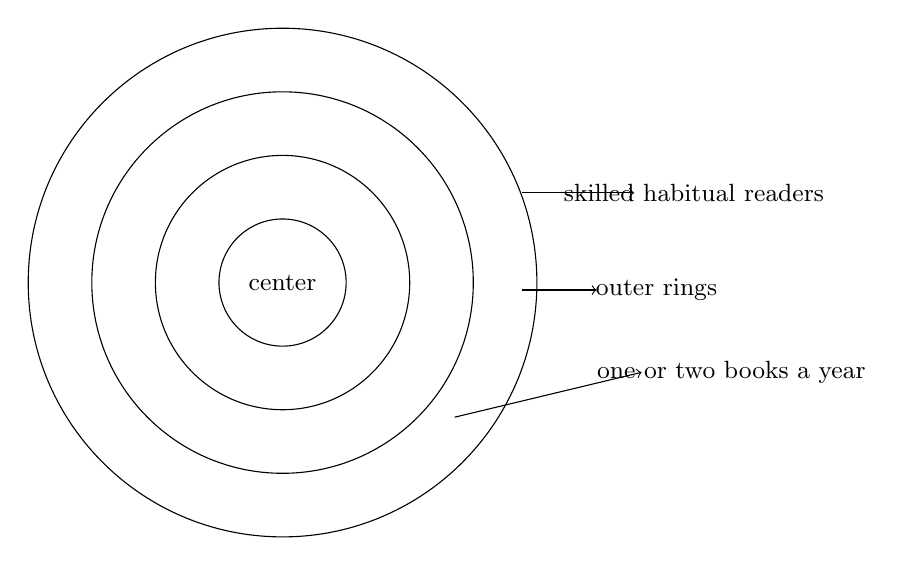
\begin{tikzpicture}[scale=0.95]
\draw (0,0) circle (0.85);
\draw (0,0) circle (1.7);
\draw (0,0) circle (2.55);
\draw (0,0) circle (3.4);
\node at (0,0) {\small center};
\node at (5.5,1.2) {\small skilled habitual readers};
\draw[->] (3.2,1.2) -- (4.7,1.2);
\node at (5.0,-0.1) {\small outer rings};
\draw[->] (3.2,-0.1) -- (4.2,-0.1);
\node at (6.0,-1.2) {\small one or two books a year};
\draw[->] (2.3,-1.8) -- (4.8,-1.2);
\end{tikzpicture}
\end{figure}

したがって design constraint は、
\begin{equation}
\text{style は center を satisfy しなければならない} \quad \& \quad \text{style は outskirts を carry しなければならない}.
\end{equation}
となる。

\subsection{Question \& Answer}

\paragraph{質問.} expert readers と、ほとんど本を読まない人たちの両方に向けて、どう write するのか。

\paragraph{答え.} two books を write することによってではない。one style に double duty をさせることによってである。center では、その style は style \emph{as} style として appreciated されうる。outskirts では、その style は useful でなければならない。guide し、ease し、carry しなければならない。Child 自身の image は physical である。writer の hand が gently に reader の back に置かれ、pressure を pressure として feel させることなく、その reader を book の through へ push していくかのようだ。

この exact point において、lecture は propulsion を introduce する。book は one sentence ではなく、sequence に置かれた thousands of sentences である。したがって local law は、
\begin{equation}
\text{sentence rhythm}_1 \to \text{sentence rhythm}_2 \to \cdots,
\qquad
\Delta p_{\text{sentence}} > 0 \text{ small but persistent}.
\end{equation}
となる。ここで \(p\) は merely an editorial name for forward pressure である。lecturer の point は simpler だ。each sentence は forward に trip しなければならない。その increase は subtle で、almost hidden である。Child はそれを、go とともに tempo が slightly accelerate する pop song に compare する。あるいは、一度 inside に入ったら elegant に exit することのできない polished carnival chute に compare する。

だからこそ、彼がもっとも value する compliments の一つは、so concrete なのである。``I finished it.'' habitual reader にとっては modest に sound するかもしれない。outer-ring reader にとっては、real achievement として register するかもしれない。したがって propulsion は、merely stylistic virtue ではない。reader を all the way through まで get する mechanics なのである。

\section{question engines、cliffhangers、そして dialogue illusion}

ひとたび propulsion が named されると、host は lecture の next useful service を perform する。propulsion を single grand word のままにしておかない。より smaller な mechanisms へそれを press していく。それは only sentences に live するのか。それとも questions にも、chapter endings にも、known であるものと not yet known であるものとの between に held-open された gap にも live するのか。Child は、prose から television へ back し、それから again prose へ戻ることで answer する。

\subsection{Question \& Answer}

\paragraph{質問.} questions と rhythm は、actual にどうやって reader を book の through へ pull するのか。

\paragraph{答え.} lack を activate することによってである。ひとたび real question が planted されると、audience はその answer を want する。その desire が、そのあと time を across し、breaks を across し、chapters を across して attention を carry する。

basic chain は、
\begin{equation}
\text{implied question} \Longrightarrow \text{answer withheld} \Longrightarrow \text{reader / viewer retention}.
\end{equation}
である。

それから host の cliffhangers に関する question が、Child に mechanism を historically derive させる。
\begin{equation}
\text{switching cost} \downarrow \Longrightarrow \text{need for sharper hooks} \uparrow.
\end{equation}

worked derivation は、この lecture でもっとも clear なものの一つである。
\begin{enumerate}
\item earlier の television world では、channel を leave するには real effort が cost した。
\item その friction が inertia を create していた。viewer は、changing channels が inconvenient である merely その理由で、break を through stay したかもしれない。
\item remote control が、その switching cost を collapse させた。
\item cost が fall すると、inertia は no longer attention を protect しなくなった。
\item したがって producers は、break の前に live question を place し、その answer を delay しなければならなくなった。
\item same principle は fiction へ transfer する。chapter ending は、merely pause ではなく、tension の under にある question になる。
\end{enumerate}

Child は、その point を performing することによって dramatize する。1990 までに viewers は、1980 には持っていなかった something を possessed するようになった、と彼は言う。host も、私たちも、いまやその answer を want している。appetite が active になった after にのみ、answer が arrive する。remote control である。だからこそ Child は conclude する。この restricted and technical sense においては、plotting difficulty は often overestimated されている、と。ひとたび genuine question が posed されれば、reader はその answer を learn するために stay するのである。

それから lecture は、その effect を mechanics から experience へ widen する。good book は、reader にそれを put down することを angry に feel させ、return することを eager に feel させる。Child は Christmas anecdote を offer する。family schedule が delayed してくれれば、自分は keep reading できるのに、と half-wished したという話である。host は、その state に right word を与える。absorption である。Child は、自分の preferred word で answer する。immersion である。point は merely speed ではない。leave しがたい world を作ることなのだ。

この stage で host は、seemingly opposite な principle を introduce する。perhaps way to achieve this は、too hard に try しないことなのではないか。Child は agree する。David Mamet の actors に関する account を cite する。actors は、liked されたいと ask しながら stage に上がるのではなく、in effect, take me or leave me と言う self-possession をもって arrive するのだ、と。同じことが writing にも apply する。likability は、too explicitly に designed されると neediness になる。

それから host は、この chapter が keep しなければならない question を ask する。そのような insouciance は、discipline とどうやって coexist するのか。Child の answer は、この lecture でもっとも explicit な paradox である。
\begin{equation}
\text{writing as art} = 100\%, \qquad
\text{writing as job} = 100\%.
\end{equation}
彼はこれを mathematically impossible と呼ぶ。そして precisely そこが point なのである。writer は、both propositions を wholly に believe しなければならない。work は artistic tradition に belong しているということと、work は family、publisher、retailer、reader の all が obligations を create する job だということを。この paradox は afterthought ではない。whole lecture の beneath にある emotional and practical structure なのである。

conversation が later に smaller scale で restart するとき、host は plot や audience からではなく main character から begin する。question は likability である。Child の answer は、Mamet principle と perfectly continuous である。main character は hated されるよう engineered されてもならない。だが liked されるよう successfully engineered されることもまたできない。matter するのは authenticity である。Reacher は、Child が initially conceived した as such において、多くの respects で barbarian だった。clue は単純に、Child が彼を liked したということだった。readers は share する culture のほうが、share しない culture より more 多いのだから、この private response は proof ではないにせよ、plausible signal ではあった。

\subsection{Question \& Answer}

\paragraph{質問.} prose を motion と emphasis のために actual に engineering しながら、どうすれば natural に feel させられるのか。

\paragraph{答え.} literal transcription は realism ではない、ということを remember することによってである。real speech は disordered である。したがって written dialogue は artificial でなければならない。だが、その artificiality は、reader がそれを natural と experience するような artificiality でなければならない。

Child はこの principle を great force をもって state する。
\begin{equation}
\text{real speech} \neq \text{written dialogue},
\qquad
\text{written dialogue is structured artifice that must feel unstructured}.
\end{equation}

real conversation は、fragments、placeholders、false starts、long dead spaces に full である。だが、それを faithfully に copied したなら、page は live しない。したがって craft problem は、speech を record することではなく、speech の illusion を construct することなのである。rhythm がその work の part を担う。stress がその work の part を担う。repetition もそうである。

host の train anecdote は、Child に explicit な example を与える。
\begin{equation}
\text{``I need my money''}, \qquad \text{``I lost my money''}
\Longrightarrow
\text{need / lost / money が stress points として rise する.}
\end{equation}

derivation は simple で exact である。
\begin{enumerate}
\item repeated noun である \emph{money} が ear に stay する。
\item emotional state が ornamental な language を strip away する。
\item verbs である \emph{need} と \emph{lost} が、pressure の change を carry するようになる。
\item resulting line は、より carefully に controlled されている precisely ゆえに、より spoken に sound する。
\end{enumerate}

Child は useful な technical caution を add する。one may use italics for emphasis in extremis ではある。だが italics が peppered された page は、soon typographical noise になってしまう。better なのは、その intended word に by itself line が land するよう rhythm を construct することだ。ここで propulsion との continuity が visible になる。chapter level においても、sentence level においても、dialogue の inside においても、task は同じである。machinery を exposing せずに pressure を engineer することなのだ。

\section{beginnings、endings、そして head の中の monster outline}

lecture はここで again broaden する。だが revealing な仕方でである。host は、book における beginnings と endings について ask する。Child は first に、life の scale で answer する。most aspiring writers は、too early なのだ、と彼は言う。enthusiasm と talent は may be present している。だが content はまだ there にない。one should read, live, accumulate. そして only then、smaller question が return する。book 自体はどこで begin し、どこで stop するのか。

rules は severe で memorable である。
\begin{equation}
\text{do not start when the earth cooled} \Longrightarrow \textit{in medias res},
\end{equation}
\begin{equation}
\text{story over} \Longrightarrow \text{book over}.
\end{equation}

前者は、live な present を explanatory な backstory の under に bury してしまう novice habit を attack する。私たちに first に everything は要らない。active な something now が必要なのだ。後者は、closure がすでに occurred したあとでも wrapping を keep したがる equally novice な impulse を attack する。Child は striking な example を give する。自分にはまだ more to write があると believe していたのに、suddenly book はすでに ended していたと realize した、というのである。

それから lecture は、different angle から television を revisit する。television が concentrated activity であることを cease し、parallel activity になってしまうと、producers は redundancy によって distraction を compensate し始めた。これから tell しますよと言い、tell し、そして told したことを tell するのである。Child は、その habit を too much prose に carry してしまう temptation を recognize した。そこで彼は、reader に more inferential work を leave するようになった。information は present であり、plain でさえある。だが final assemblage は、always page の上で performed されるわけではない。

この turn が matter するのは、それが lecture の next answer を prepare するからである。もし one leaves more work to the reader なのだとしたら、one is relying on structure していることになる。だが、その structure は 어디にあるのか。outline の中にないのだとしたら。

\subsection{Question \& Answer}

\paragraph{質問.} written outline がないなら、structure はどこから come するのか。

\paragraph{答え.} many thousands of prior structures の internalization からである。Child の point は、彼が form なしに create しているということではない。form はすでに absorbed されている、ということなのだ。reading がそれを installed したのである。

この claim は、
\begin{equation}
\text{read された tens of thousands of books} \Longrightarrow \text{plots, characters, cliffhangers, structures の internal database}.
\end{equation}
と書ける。

したがって、more careful な reconstruction は
\begin{equation}
\text{improvisation} + \text{massive prior reading} \Longrightarrow \text{implicit structural control}.
\end{equation}
となる。

だからこそ ``monster outline'' という phrase は so useful なのである。Child は paper outline を deny する。だが internal one を affirm する。host はここで help する。他の arts から analogies を supply することによってである。designers、musicians、filmmakers、all of them outsiders suppose するより far more consume しているのだ、と。Child は immediately にその diagnosis を confirm する。writers は primarily writers ではない。primarily readers なのである。

彼の late ratio は、その point を almost comic clarity で make する。
\begin{equation}
\text{books written per year} \ll \text{books read per year}.
\end{equation}

それが no-outline puzzle への answer なのである。structure は absent なのではない。memory、habit、genre knowledge、long exposure の through に distributed されているのである。drawing が spontaneous に feel される even ときも、writer は immense filing system から drawing しているのだ。

\section{violence、character shorthand、そして teaching の limits}

final movement は、at first sight には miscellaneous に見える several topics を gather する。だがそうではない。each は same thesis へ return する。fiction は literal copying によってではなく、stylized selection によって work するのだ、という thesis へ。

violence は clearest late example である。Child は、narrative における violence は、once again, illusion だと言う。real violence は usually brief で、ungainly で、significant after-effects を followed by する。blows が exchanged され、しかも endless recoverability とともに行ったり来たりする screen version は、almost never realistic ではない。ではなぜ reader はそれを want するのか。lecture は paradox によって answer する。

\begin{equation}
\text{civilized commitment to due process} + \text{private retaliatory desire}
\Longrightarrow
\text{fictional violence as release}.
\end{equation}

readers は law、safeguards、rights、civilization を believe している。real world が vengeance を軸に reorder されることは want していない。だが、private な retaliatory desire の flash も know している。fiction は、その protected conditions の under で release を offer する。reader は world が fictional だと know している。したがって、その satisfaction を socially inhabit したいわけではなくても enjoy できる。violence section の transcript は partially garbled だが、その stable structure は sufficiently clear である。real violence は brief で costly である。fictional violence は、documentary fidelity ではなく psychic release を serving しているがゆえに stylized されているのだ。

same selective logic は、それから characterization に appear する。clothing、shoes、hair、teeth。これらは fast visual operators になる。gray ponytail with double denim でも、あるいは lace-up shoes と pleated chinos の opposite stiffness でも、人は quickly に place されうる。teeth も同じことをしうる。Child は、自分は dentist reader がそれに notice させるまで、instinctively にそれを doing していたのだと remark する。technical point は、character が wardrobe や dentition に reduce されるということではない。fiction は often efficient で high-yield な signals を need とする、ということなのである。

\subsection{Question \& Answer}

\paragraph{質問.} writing は actual に taught されうるのか。それとも only long exposure を通じて learned されるものなのか。

\paragraph{答え.} Child は real distinction を draw する。writing のまわりにある much は certainly taught されうる。business、pitfalls、professional handling などである。だが central art は、彼の view では straightforwardly teachable ではない。それでも nonetheless learnable ではありうる。one can read, listen, live, and slowly internalize what no short formula could successfully hand over.

この answer は、entire lecture に fit している。dialogue は listening によって learned される。structure は reading によって learned される。character は watching によって sharpen される。national storytelling cultures に関する final answers ですら、私たちをこの point へ return させる。Child の account において Scotland は、power の concentration に against して alternative culture を build する。Ireland は別の something を provide する。chance を与える gift である。pub で story を begin telling したなら、room は judging する before に few seconds を hear してくれる。その small allowance は culturally enormous である。それは storyteller を train する。floor を seize し、それを quickly justify し、keep し続けるように。

したがって lecture は、rule の上で close するのではなく、growth の condition の上で close する。storys、forms、listeners に dense な world の中へ enter し、それらに answerable になることによって、人は writing を learn するのである。

\section{Summary}

lecture の order それ自体が lesson である。私たちは scale から begin する。scale が immediately plausibility の problem を raise するからである。そこから geography へ move し、geography から temperature と key としての place へ move し、place から anti-outline claim へ move する。improvisation はそれから emptiness ではないことが prove される。reading に backed された mode なのである。lecture はそこから audience、transaction、readership の rings へ again widen し、その widened view から propulsion、question-hooks、cliffhangers、sentence の pressure を derive する。そして locally に character と dialogue へ restart したのち、beginnings、endings、violence、shorthand characterization、teaching の limits へ once more outward に move する。

もっとも strong な unifying claim は、writing は never one thing only ではない、ということである。それは local であり large-scale でもあり、spontaneous であり disciplined でもあり、readerly であり writerly でもあり、artistic であり occupational でもある。だからこそ closing paradox は decorative ではなく exact なのである。Child は、apparently incompatible な two truths を at once hold するよう私たちに ask する。そして whole lecture は、それがどうやって done されうるのかの extended demonstration だったのである。